\section{Durchführung}
\label{sec:Durchführung}

Die Temperaturabhängigkeit des Dampfdruckes soll im Bereich $50\,\unit{\milli\bar}$ bis $15\,\unit{\bar}$
gemessen werden.
Dafür muss für die niedrigen Drücke unter $1\,\unit{\bar}$ ein anderer Versuchsaufbau als für die hohen
Drücke über $1\,\unit{\bar}$ verwendet werden.

\subsection{Messung bis 1 bar}
\label{sec:Messung bis 1 bar}

Im ersten Versuchsteil wird die Messung für kleine Drücke durchgeführt.
Der verwendete Versuchsaufbau ist in \autoref{fig:Versuchsaufbau 1bar} dargestellt.

Zuerst wird die Apperatur mit der Wasserpumpe nahezu vakuumiert, sodass ein Druck unter $50\,\unit{\milli\bar}$ gemessen wird.
Anschließend erhitzt die Heizhaube das Wasser im Mehrhalskolben ausgehend von $20\,\unit{\celsius}$ solange, bis ein Dampfdruck
von $1\,\unit{\bar}$ erreicht wird.
Dabei wird in Abständen von $2\,\unit{\celsius}$ der jeweilige Dampfdruck abgelesen und notiert.

\begin{figure} [H]
    \centering
    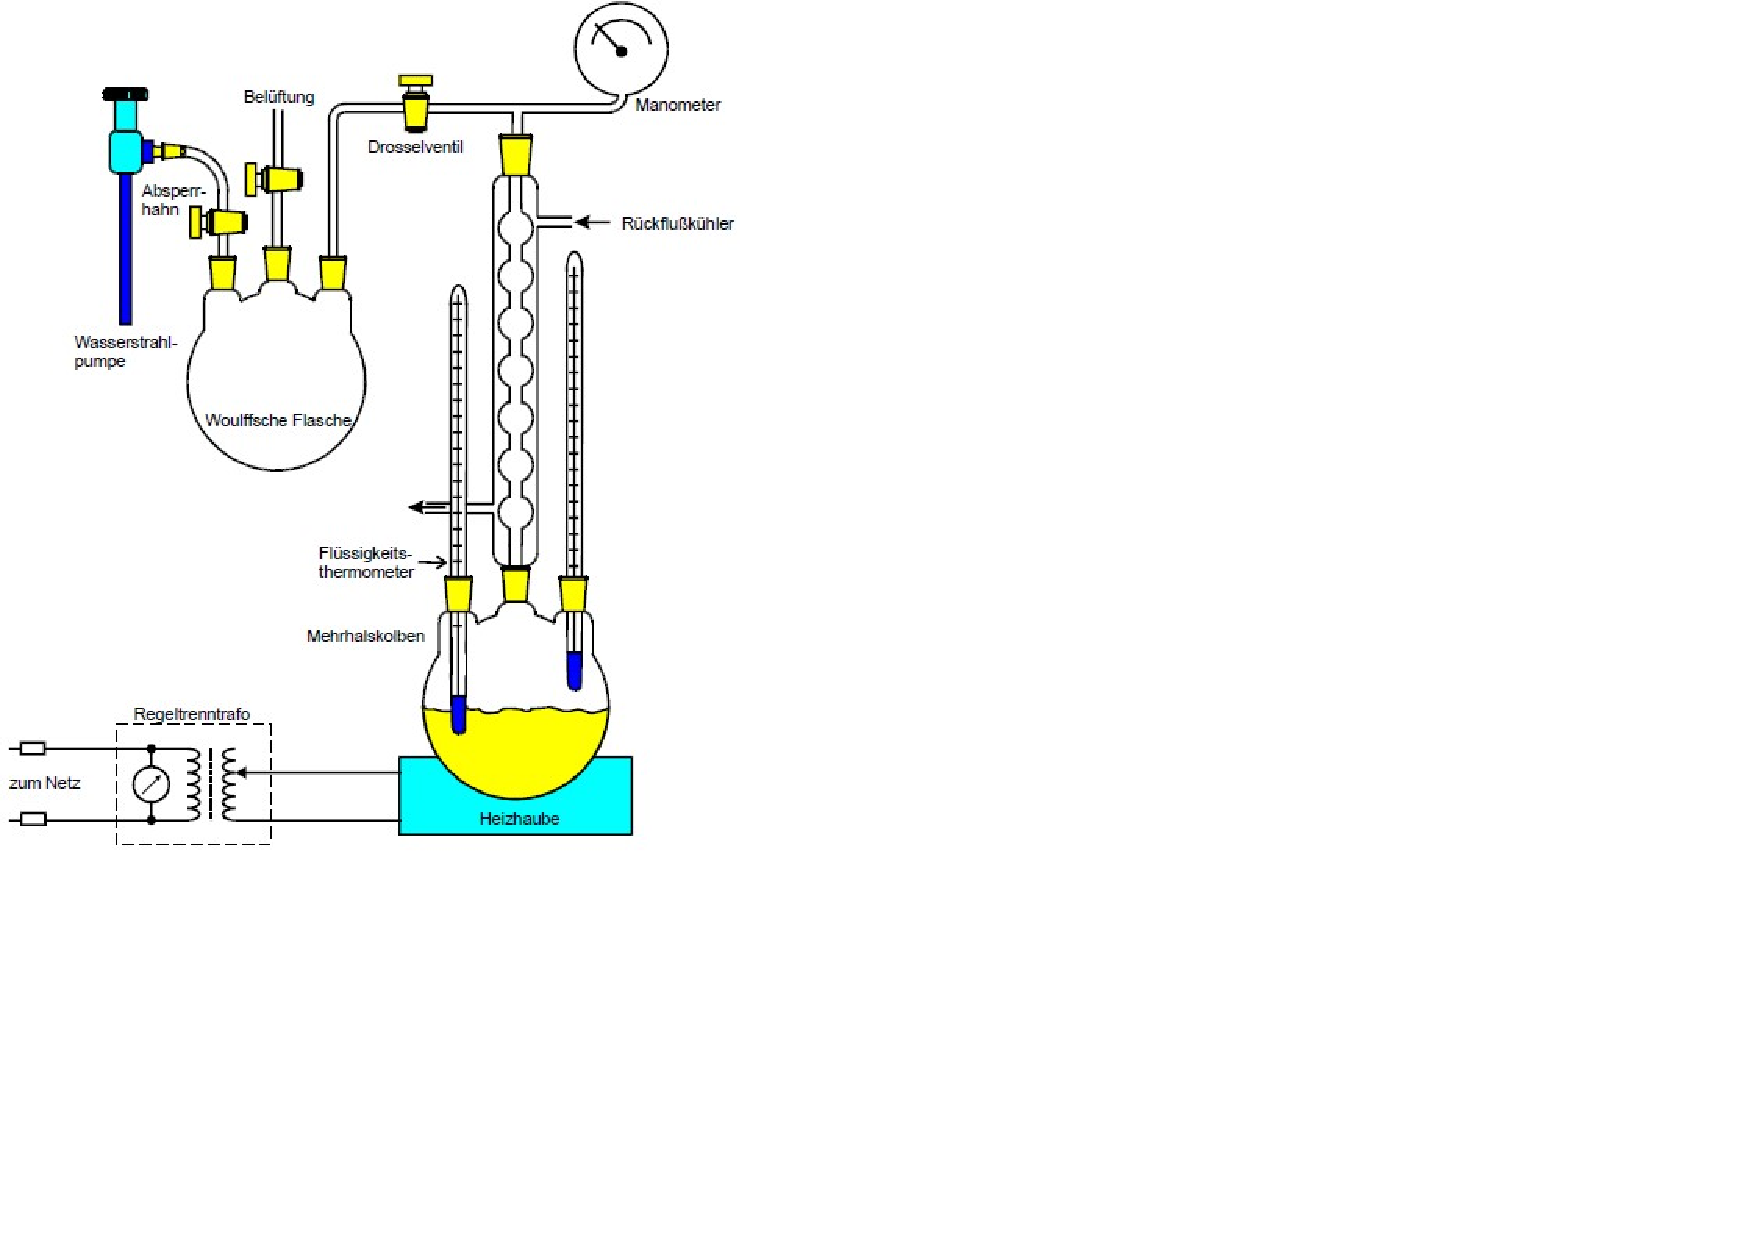
\includegraphics[height=8cm]{content/Bilder/Versuchsaufbau_1bar.pdf}
    \caption{Versuchsaufbau für kleinen Druck unter 1 bar. \cite{v203}}
    \label{fig:Versuchsaufbau 1bar}
\end{figure}

\subsection{Messung von 1 bis 15 Bar}
\label{sec:Messung von 1 bis 15 Bar}

Im zweiten Versuchsteil werden nun die höheren Drücke betrachtet.
Der neue Versuchsaufbau ist in \autoref{fig:Versuchsaufbau 15bar} zu sehen.

Die Heizwicklung wird eingeschaltet und das Wasser im Kolben erhitzt.
Sobald $1\,\unit{\bar}$ Dampfdruck erreicht ist, wird die Temperatur das erste mal abgelesen und festgehalten.
Anschließend wird dies in $1\,\unit{\bar}$ Schritten wiederholt, bis der angestrebte Druck
von $15\,\unit{\bar}$ erreicht wird.

\begin{figure} [H]
    \centering
    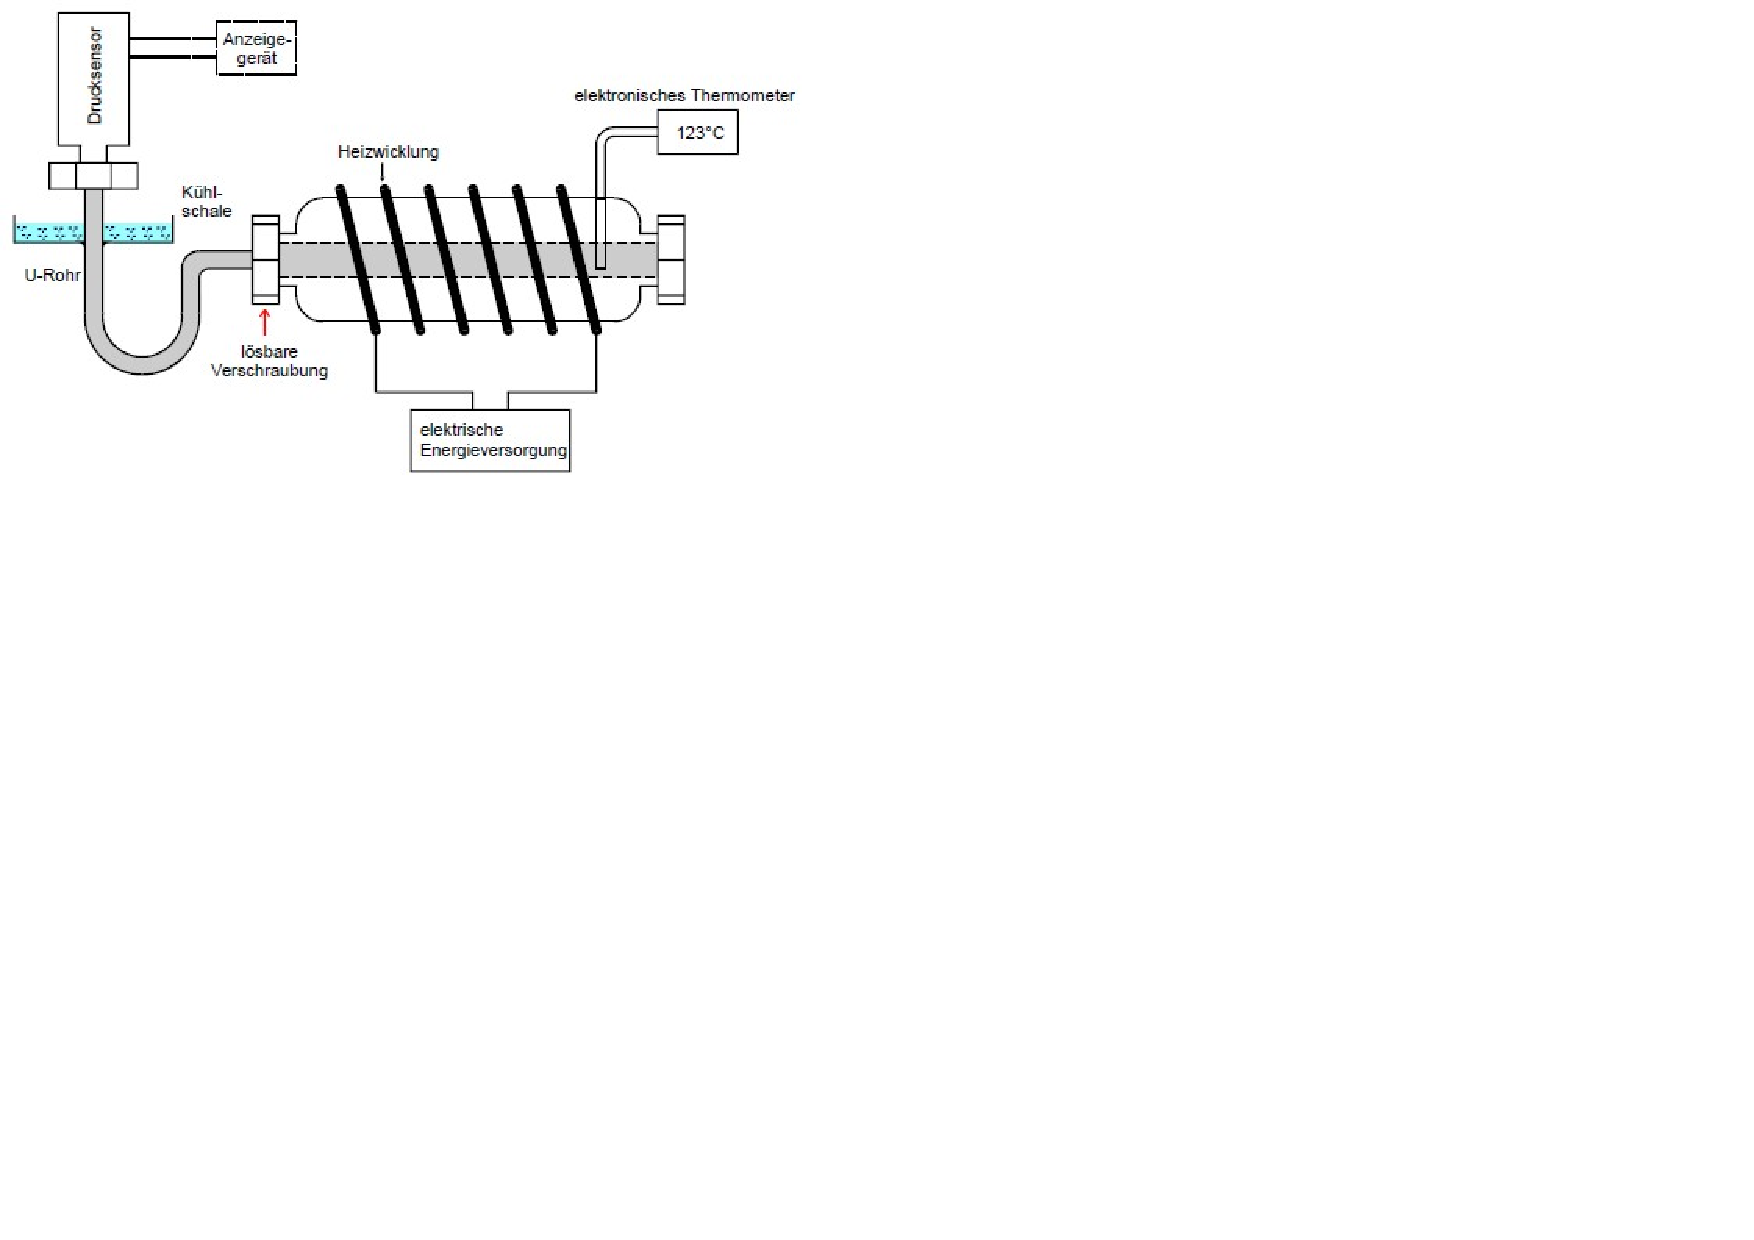
\includegraphics[height=6cm]{content/Bilder/Versuchsaufbau_15bar.pdf}
    \caption{Versuchsaufbau für großen Druck bis 15 bar. \cite{v203}}
    \label{fig:Versuchsaufbau 15bar}
\end{figure}